\documentclass{article}
  
\usepackage[utf8]{inputenc}
\usepackage[french]{babel}
\usepackage{mathtools}
\usepackage{graphicx}
\usepackage{amsmath,amssymb}
\renewcommand{\contentsname}{Sommaire}


%%%%%%%%%%%%%%%% Lengths %%%%%%%%%%%%%%%%
\setlength{\textwidth}{15.5cm}
\setlength{\evensidemargin}{0.5cm}
\setlength{\oddsidemargin}{0.5cm}

%%%%%%%%%%%%%%%% Variables %%%%%%%%%%%%%%%%
\def\projet{2}
\def\titre{M\'ethode du gradient conjugu\'e / Application \`a l’\'equation de la chaleur}
\def\groupe{1}
\def\equipe{3}
\def\responsible{mbailleul001}
\def\secretary{mzizi001}
\def\others{amdahmani, ndo001, helfani}

\begin{document}

%%%%%%%%%%%%%%%% Header %%%%%%%%%%%%%%%%
\noindent\begin{minipage}{0.98\textwidth}
  \vskip 0mm
  \noindent
  { \begin{tabular}{p{7.5cm}}
      {\bfseries \sffamily
        Projet \projet} \\ 
      {\itshape \titre}
    \end{tabular}}
  \hfill 
  \fbox{\begin{tabular}{l}
      {~\hfill \bfseries \sffamily Groupe \groupe\ - Equipe \equipe
        \hfill~} \\[2mm] 
      Responsable : \responsible \\
      Secr\'etaire : \secretary \\
      Codeurs : \others
    \end{tabular}}
  \vskip 4mm ~

  ~~~\parbox{0.95\textwidth}{\small \textit{R\'esum\'e:} \sffamily Ce projet s'int\'eresse \`a la r\'esolution des \'equations lin\'eaires. Il traite sp\'ecifiquement le cas des matrices sym\'etriques d\'efinies positives et creuses. La premi\`ere partie s'int\'eresse \`a la d\'ecomposition de Cholesky des matrices S.D.P. La deuxi\`eme partie cherche \`a r\'esoudre un syst\`eme lin\'eaire en utilisant la m\'ethode du gradient conjugu\'e. La troisi\`eme partie utilise les r\'esultats des parties pr\'ec\'edentes pour r\'esoudre des cas sp\'ecifiques de l'\'equation de chaleur en la transformant en syst\`eme lin\'eaire.}
  \vskip 1mm ~
\end{minipage}

%%%%%%%%%%%%%%%% Main part %%%%%%%%%%%%%%%%

\tableofcontents

\newpage
\section{D\'ecomposition de Cholesky}
\subsection{R\'esolution d'un syst\`eme lin\'eaire}
La d\'ecomposition de Cholesky d'une matrice A sym\'etrique d\'efinie positive consiste \`a trouver une matrice L triangulaire telle que : $A = LL^T$. Nous avons r\'eussis \`a impl\'ementer cette d\'ecomposition en algorithme de complexit\'e temporelle $O(n^3)$ ($n$ \'etant la taille de la matrice $A$). Apr\`es avoir trouv\'e la matrice $L$ la r\'esolution d'un syst\`eme lin\'eaire $Ax=b$ se traduit de la façon suivante :
\begin{center}
    $LL^Tx=b \Longleftrightarrow 
        \begin{cases*}
            Ly=b\\
            L^Tx=y\\
        \end{cases*}
    $
\end{center}
La r\'esolution de ces deux syst\`emes est simple puisque les deux matrices $L$ et $L^T$ sont triangulaires. Nous avons r\'eussi \`a l'impl\'ementer en une complexit\'e de $O(n^2)$. La r\'esolution du syst\`eme $Ax=b$ se fait donc en une complexit\'e totale de $O(n^3)$.
\subsection{G\'en\'erateur de matrices S.D.P}
Pour g\'en\'erer des matrices sym\'etriques d\'efinies positives creuses, nous avons d'abord commenc\'e par g\'en\'erer une matrice diagonale \`a coefficients al\'eatoires strictement positives. Nous commençons ensuite \`a injecter des coefficients extra-diagonaux al\'eatoires non nuls de façon sym\'etrique tout en v\'erifiant que la matrice reste d\'efinie positive. Si ce n'est pas le cas nous enlevons les coefficients que nous venons d'ins\'erer et nous recommencons. Cela continue jusqu'\`a l'obtention du nombre de coefficients extra-diagonaux non nuls demand\'e.

Pour \'eviter que cet algorithme ne se termine jamais dans des cas o\`u il est impossible de construire une matrice S.D.P avec les coefficients ins\'er\'es dans les \'etapes pr\'ec\'edentes, s'il d\'epasse un certain nombre d'it\'erations (Nous avons choisi 10 fois le nombre de coefficients extra-diagonaux non nuls) l'algorithme abandonne la matrice qu'il est en train de construire et recommence.
\subsection{D\'ecomposition de Cholesky incompl\`ete}
La version incompl\`ete de Cholesky ignore le calcul de certains \'el\'ements afin de diminuer sa complexit\'e temporelle ($O(m)$ o\`u $m$ est le nombre de coefficients non nuls de la matrice au lieu de $O(n^2)$). Cette r\'eduction se fait au prix de l'approximations du r\'esultat final.
Avec cette m\'ethode, la r\'esolution du syst\`eme lin\'eaire se fait en $O(m*n)$.

\subsection{Pr\'econditionneur}
Pour tester la qualit\'e de $M=LL^T$ comme pr\'econditionneur, nous avons compar\'e $cond(M^{-1}A)$ et $cond(A)$. Nous avons obtenu les r\'esultats suivants :
\begin{center}
\begin{tabular}{|l|c|c|c|c|c|c|c|}
  \hline
  $cond(M^{-1}A)$ dense & $\sim1$ & $\sim1$ & $\sim1$ & $\sim1$ & $\sim1$ & $\sim1$ & $\sim1$ \\
  \hline
  $cond(M^{-1}A)$ incompl\`ete & 10.7 & 127.5 & 5.95 & 308.39 & 232.52 & 2204.87 & 660.95 \\
  \hline
  $cond(A)$ & 1484.3 & 1536.2 & 25.9 & 1241.06 & 909.66 & 8571.31 & 7213.5 \\
  \hline
\end{tabular}
\end{center}
Dans tous ces cas, on a pour Cholesky incompl\`ete : $cond(M^{-1}A) < cond(A)$. Cette m\'ethode produit donc des pr\'econditionneurs de bonne qualit\'e.
\subsection{Les tests}
\begin{itemize}
    \item Les tests des fonctions $cholesky\_dense()$ et $cholesky\_incomplete()$ consistent \`a choisir une vari\'et\'e de matrices $A$ (enti\`ere, flottante et identit\'e) et de g\'en\'erer leur d\'ecomposition respectives $L$. Nous v\'erifions ensuite que $L$ est triangulaire (m\^eme inf\'erieur dans notre cas) et que $LL^T=A$.
    \item Pour le g\'en\'erateur de matrices S.D.P, nous avons cr\'e\'e une fonction $is\_positive\_definite()$ qui d\'etermine si une matrice est d\'efinie positive en calculant les d\'eterminants de ses sous-matrices.
    \item Pour la fonction $solve\_cholesky()$, on compare les r\'esultats qu'elle fournit sur diff\'erentes matrices avec les r\'esultats de la fonction $numpy.linalg.solve()$ de numpy.
\end{itemize}
\section{M\'ethode du gradient conjugu\'e}
\subsection{Principe}
Au contraire de la m\'ethode Cholesky, pour r\'esoudre les syst\`emes lin\'eaires, la m\'ethode du gradient conjugu\'e prend un vecteur de d\'epart $x$ et le modifie graduellement pour converger vers la solution. Cette m\'ethode peut donc s'arr\^eter \`a n'importe quel moment pour donner une valeur approximative de la solution.
\subsection{D\'efauts de l'algorithme propos\'e}
L'algorithme propos\'e contient un $if(A):break$ \`a l'int\'erieur d'une boucle $for$ ce qui (bien que fonctionnel) ne respecte pas les standards du codage tr\`es sains. Une solution alternative est de remplacer la boucle $for$ par une boucle $while$ ayant deux conditions d'arr\^et :
\begin{center}
    \begin{tabular}{|l|}
        \hline 
        \vdots\\
        $rnew = 1$\\
        $i=0$\\
        $while(sqrt(rsnew) > 1e-10$ $and$ $i < 10e6):$\\
        \hspace{5mm} \vdots\\
        \hspace{5mm} $i+=1$\\
        \vdots\\
        \hline
    \end{tabular}
\end{center}
Le choix de la valeur initiale de $rnew$ est arbitraire et n'affecte pas l'ex\'ecution de l'algorithme. Il faut juste que cette valeur permette une premi\`ere ex\'ecution de la boucle $while$.

\subsection{Pr\'econditionnement}
Pour acc\'el\'erer l'algorithme pr\'ec\'edent, nous avons impl\'ement\'e la m\'ethode avec pr\'econditionnement. Vu les r\'esultats de la premi\`ere partie, nous avons pris comme pr\'econditionneur $LL^T$ avec $L$ le r\'esultat de la d\'ecomposition de Cholesky.
Nous avons compar\'e la vitesse des versions avec et sans pr\'econditionnement en prenant comme r\'ef\'erence la norme du vecteur $r$ \`a chaque it\'eration puisqu’elle d\'etermine l'arr\^et de l'algorithme.

\begin{figure}[!ht]
    \centering
    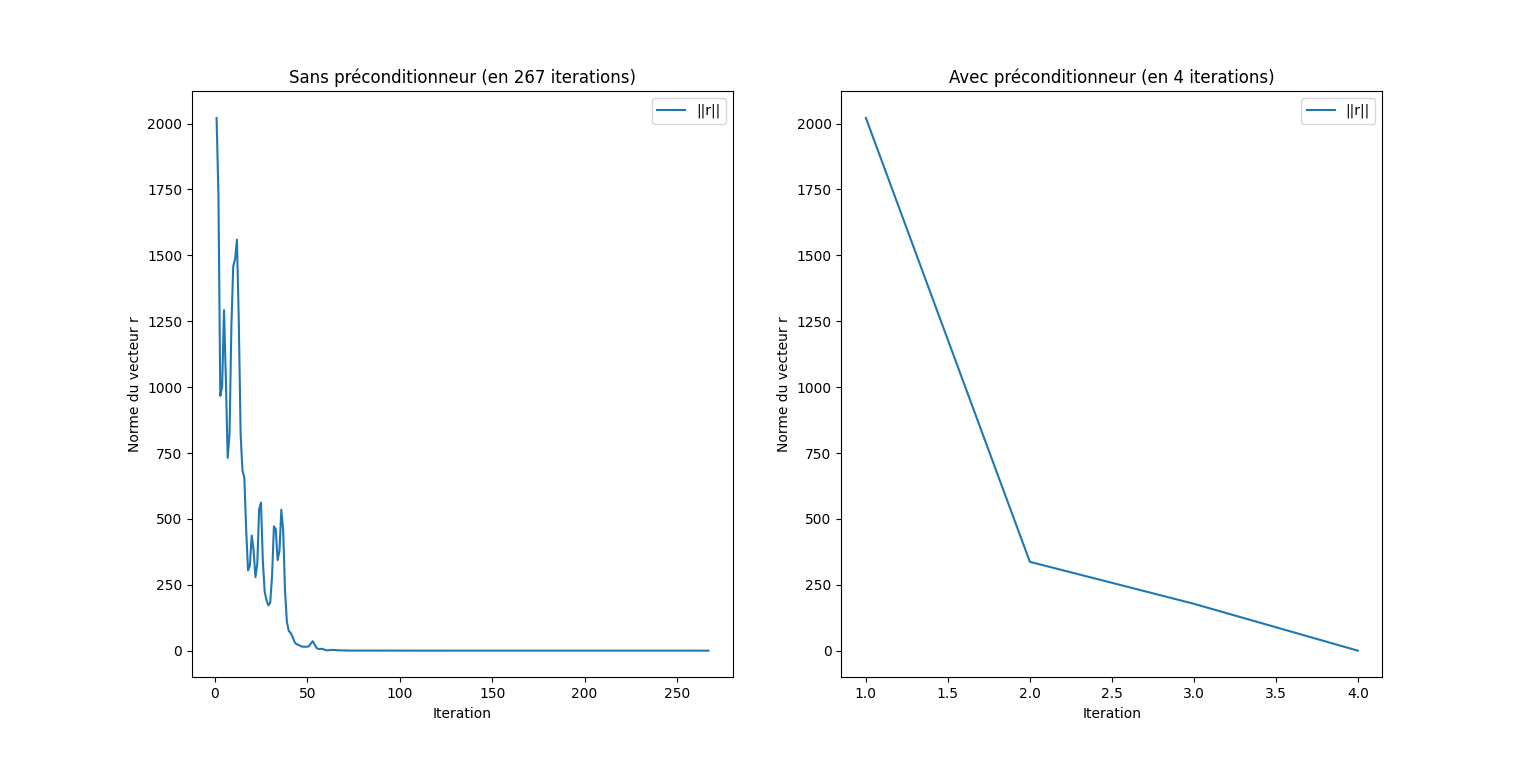
\includegraphics[width=0.7\textwidth]{precond.png}
    \caption{Vitesse de convergence avec et sans pr\'econditionnement}
    \label{fig:1}
\end{figure}

La figure \ref{fig:1} montre clairement l'avantage qu'apporte la version avec pr\'econditionnement, celle-ci se terminant en 4 it\'erations alors que la version initiale en prend 267.

\subsection{Les tests}
Comme pour la fonction $solve\_cholesky()$ de la partie pr\'ec\'edente, on compare ici les r\'esultats de nos deux m\'ethode avec ceux de la fonction $numpy.linalg.solve()$ de numpy.
\section{\'equation de la chaleur}
\subsection{Forme matricielle}
On essaye de trouver une solution $T$ \`a l'\'equation :
\begin{center}
$\frac{\partial^2T}{\partial x^2} + \frac{\partial^2T}{\partial y^2} = f(x, y)$\\
\end{center}
En posant les matrices suivantes : $\forall(i,j) \in [\![ 0~;~ N-1 ]\!]^2$
\begin{center}
\begin{tabular}{l l l}
$T,F \in \mathcal{M}_{N^2, 1}(\mathbb{R}),$&$T_{i*N + j} = T(x_i, y_j)$&$F_{i*N + j} = f(x_i, y_j)$\\
\end{tabular}
\end{center}
Et en approximant la d\'eriv\'ee seconde comme suit :
\begin{center}
$f''(x) = \frac{f(x + h) + f(x - h) - 2f(x)}{h^2}$\\
\end{center}
L'\'equation devient : $\forall(i,j) \in [\![ 1~;~ N-2 ]\!]^2$
\begin{center}
$\frac{T_{(i+1)N + j} + T_{(i-1)N + j} + T_{iN + (j + 1)} + T_{iN + (j - 1)} - 4T_{iN + j}}{h^2} = F_{iN + j}$\\
\end{center}
(Remarque : Pour respecter les conditions aux bords, on prend 0 au lieu des termes $T_{(i-1)N + j}$, $T_{(i+1)N + j}$, $T_{iN + j-1}$ et $T_{iN + j+1}$ si $i = 0$, $i = N - 1$, $j = 0$ ou $j = N - 1$ respectivement).\\
Supposons qu'il existe une matrice $Mc \in \mathcal{M}_{N^2, N^2}(\mathbb{R})$ v\'erifiant :
\begin{center}
$\frac{1}{h^2} Mc * T = F$\\
\end{center}
En calculant le produit matriciel on obtient : $\forall(i,j) \in [\![ 1~;~ N-2 ]\!]^2$
\begin{center}
$\frac{1}{h^2} \sum_{k=0}^{N^2 - 1} (Mc_{iN+j,k} * T_{k}) = F_{iN + j}$\\
\bigskip
$\frac{1}{h^2} \sum_{k=0}^{N^2 - 1} (Mc_{iN+j,k} * T_{k}) = \frac{T_{(i+1)N + j} + T_{(i-1)N + j} + T_{iN + (j + 1)} + T_{iN + (j - 1)} - 4T_{iN + j}}{h^2}$\\
\bigskip
$\sum_{k=0}^{N^2 - 1} (Mc_{iN+j,k} * T_{k}) = T_{(i+1)N + j} + T_{(i-1)N + j} + T_{iN + (j + 1)} + T_{iN + (j - 1)} - 4T_{iN + j}$\\
\bigskip
(La remarque pr\'ec\'edente s'applique ici).\\
\end{center}
Et donc, en prenant $p = iN +j$ :
\begin{center}
$\sum_{k=0}^{N^2 - 1} (Mc_{p,k} * T_{k}) = T_{p + N} + T_{p - N} + T_{p + 1} + T_{p - 1} - 4T_{p}$\\
\end{center}
En faisant correspondre les termes $T_k$ des deux c\^ot\'es on trouve alors les coefficients de la matrice $Mc$ :
\begin{center}
$
    Mc_{p,k} =
    \begin{cases*}
      -4    & Si p = k\\
      1     & Si k $\in$ \{ p + N, p - N, p + 1, p - 1 \}  \\
      0     & Sinon
    \end{cases*}
$
\end{center}
Nous avons ainsi retrouv\'e la forme de la matrice $Mc$ propos\'ee par l'exercice. Il est important de noter pour la prochaine sous-partie que cette matrice est S.D.P.
\subsection{Application}
Puisque la r\'esolution de l'\'equation de la chaleur en r\'egime stationnaire revient \`a r\'esoudre un syst\`eme lin\'eaire $Mc*T=F$ o\`u $Mc$ est S.D.P, il suffit d'appliquer la m\'ethode de la partie pr\'ec\'edente.\\
\begin{figure}[!ht]
    \centering
    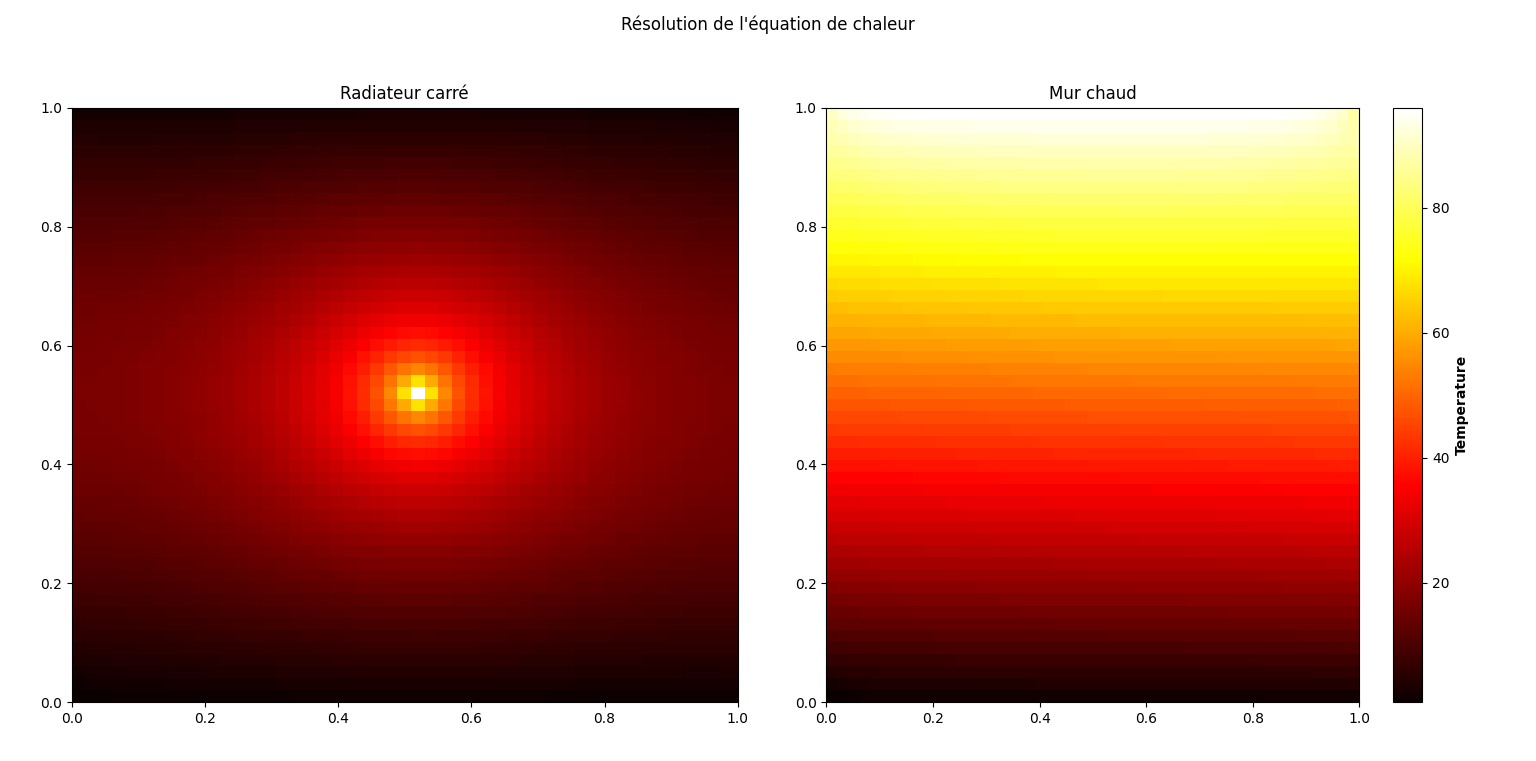
\includegraphics[width=0.7\textwidth]{chaleur_c.png}
    \caption{R\'esolution de l'\'equation de chaleur}
    \label{fig:2}
\end{figure}

La matrice $F$ ici repr\'esente les sources de chaleur (en signe n\'egative). Pour simuler les cas demand\'es il faut choisir $F$ \`a coefficients nuls sauf pour :
\begin{itemize}
\item Pour le radiateur au milieu du plan : $i = j = \left\lfloor\dfrac{N}{2}\right\rfloor$, $F_{iN +j}= -temp$
\item Pour le mur chaud au nord : $\forall j \in [\![ 0~;~ N-1 ]\!],$ $F_{(N-1)N + j}= -temp$
\end{itemize}

La figure \ref{fig:2} montre les r\'esultats obtenus en suivant cette d\'emarche.
\end{document}
